\documentclass{ximera}
%\usepackage{todonotes}

\newcommand{\todo}{}

\usepackage{tkz-euclide}
\tikzset{>=stealth} %% cool arrow head
\tikzset{shorten <>/.style={ shorten >=#1, shorten <=#1 } } %% allows shorter vectors

\usepackage{tkz-tab}  %% sign charts
\usetikzlibrary{decorations.pathreplacing} 

\usetikzlibrary{backgrounds} %% for boxes around graphs
\usetikzlibrary{shapes,positioning}  %% Clouds and stars
\usetikzlibrary{matrix} %% for matrix
\usepgfplotslibrary{polar} %% for polar plots
\usetkzobj{all}
\usepackage[makeroom]{cancel} %% for strike outs
%\usepackage{mathtools} %% for pretty underbrace % Breaks Ximera
\usepackage{multicol}

\usepackage{polynom}



\usepackage[many]{tcolorbox}  %% for titled boxes
\newtcolorbox{xbox}[1]{%
    tikznode boxed title,
    enhanced,
    arc=0mm,
    interior style={white},
    attach boxed title to top center= {yshift=-\tcboxedtitleheight/2},
    fonttitle=\bfseries,
    colbacktitle=white,coltitle=black,
    boxed title style={size=normal,colframe=white,boxrule=0pt},
    title={#1}}


\usepackage{array}
\setlength{\extrarowheight}{+.1cm}   
\newdimen\digitwidth
\settowidth\digitwidth{9}
\def\divrule#1#2{
\noalign{\moveright#1\digitwidth
\vbox{\hrule width#2\digitwidth}}}





\newcommand{\RR}{\mathbb R}
\newcommand{\R}{\mathbb R}
\newcommand{\N}{\mathbb N}
\newcommand{\Z}{\mathbb Z}

%\renewcommand{\d}{\,d\!}
\renewcommand{\d}{\mathop{}\!d}
\newcommand{\dd}[2][]{\frac{\d #1}{\d #2}}
\newcommand{\pp}[2][]{\frac{\partial #1}{\partial #2}}
\renewcommand{\l}{\ell}
\newcommand{\ddx}{\frac{d}{\d x}}
\newcommand{\ddt}{\frac{d}{\d t}}

\newcommand{\zeroOverZero}{\ensuremath{\boldsymbol{\tfrac{0}{0}}}}
\newcommand{\inftyOverInfty}{\ensuremath{\boldsymbol{\tfrac{\infty}{\infty}}}}
\newcommand{\zeroOverInfty}{\ensuremath{\boldsymbol{\tfrac{0}{\infty}}}}
\newcommand{\zeroTimesInfty}{\ensuremath{\small\boldsymbol{0\cdot \infty}}}
\newcommand{\inftyMinusInfty}{\ensuremath{\small\boldsymbol{\infty - \infty}}}
\newcommand{\oneToInfty}{\ensuremath{\boldsymbol{1^\infty}}}
\newcommand{\zeroToZero}{\ensuremath{\boldsymbol{0^0}}}
\newcommand{\inftyToZero}{\ensuremath{\boldsymbol{\infty^0}}}



\newcommand{\numOverZero}{\ensuremath{\boldsymbol{\tfrac{\#}{0}}}}
\newcommand{\dfn}{\textbf}
%\newcommand{\unit}{\,\mathrm}
\newcommand{\unit}{\mathop{}\!\mathrm}
\newcommand{\eval}[1]{\bigg[ #1 \bigg]}
\newcommand{\seq}[1]{\left( #1 \right)}
\renewcommand{\epsilon}{\varepsilon}
\renewcommand{\iff}{\Leftrightarrow}

\DeclareMathOperator{\arccot}{arccot}
\DeclareMathOperator{\arcsec}{arcsec}
\DeclareMathOperator{\arccsc}{arccsc}
\DeclareMathOperator{\si}{Si}
\DeclareMathOperator{\proj}{proj}
\DeclareMathOperator{\scal}{scal}


\newcommand{\tightoverset}[2]{% for arrow vec
  \mathop{#2}\limits^{\vbox to -.5ex{\kern-0.75ex\hbox{$#1$}\vss}}}
\newcommand{\arrowvec}[1]{\tightoverset{\scriptstyle\rightharpoonup}{#1}}
\renewcommand{\vec}{\mathbf}
\newcommand{\veci}{\vec{i}}
\newcommand{\vecj}{\vec{j}}
\newcommand{\veck}{\vec{k}}
\newcommand{\vecl}{\boldsymbol{\l}}

\newcommand{\dotp}{\bullet}
\newcommand{\cross}{\boldsymbol\times}
\newcommand{\grad}{\boldsymbol\nabla}
\newcommand{\divergence}{\grad\dotp}
\newcommand{\curl}{\grad\cross}
%\DeclareMathOperator{\divergence}{divergence}
%\DeclareMathOperator{\curl}[1]{\grad\cross #1}


\colorlet{textColor}{black} 
\colorlet{background}{white}
\colorlet{penColor}{blue!50!black} % Color of a curve in a plot
\colorlet{penColor2}{red!50!black}% Color of a curve in a plot
\colorlet{penColor3}{red!50!blue} % Color of a curve in a plot
\colorlet{penColor4}{green!50!black} % Color of a curve in a plot
\colorlet{penColor5}{orange!80!black} % Color of a curve in a plot
\colorlet{fill1}{penColor!20} % Color of fill in a plot
\colorlet{fill2}{penColor2!20} % Color of fill in a plot
\colorlet{fillp}{fill1} % Color of positive area
\colorlet{filln}{penColor2!20} % Color of negative area
\colorlet{fill3}{penColor3!20} % Fill
\colorlet{fill4}{penColor4!20} % Fill
\colorlet{fill5}{penColor5!20} % Fill
\colorlet{gridColor}{gray!50} % Color of grid in a plot

\newcommand{\surfaceColor}{violet}
\newcommand{\surfaceColorTwo}{redyellow}
\newcommand{\sliceColor}{greenyellow}




\pgfmathdeclarefunction{gauss}{2}{% gives gaussian
  \pgfmathparse{1/(#2*sqrt(2*pi))*exp(-((x-#1)^2)/(2*#2^2))}%
}


%%%%%%%%%%%%%
%% Vectors
%%%%%%%%%%%%%

%% Simple horiz vectors
\renewcommand{\vector}[1]{\left\langle #1\right\rangle}


%% %% Complex Horiz Vectors with angle brackets
%% \makeatletter
%% \renewcommand{\vector}[2][ , ]{\left\langle%
%%   \def\nextitem{\def\nextitem{#1}}%
%%   \@for \el:=#2\do{\nextitem\el}\right\rangle%
%% }
%% \makeatother

%% %% Vertical Vectors
%% \def\vector#1{\begin{bmatrix}\vecListA#1,,\end{bmatrix}}
%% \def\vecListA#1,{\if,#1,\else #1\cr \expandafter \vecListA \fi}

%%%%%%%%%%%%%
%% End of vectors
%%%%%%%%%%%%%

%\newcommand{\fullwidth}{}
%\newcommand{\normalwidth}{}



%% makes a snazzy t-chart for evaluating functions
%\newenvironment{tchart}{\rowcolors{2}{}{background!90!textColor}\array}{\endarray}

%%This is to help with formatting on future title pages.
\newenvironment{sectionOutcomes}{}{} 



%% Flowchart stuff
%\tikzstyle{startstop} = [rectangle, rounded corners, minimum width=3cm, minimum height=1cm,text centered, draw=black]
%\tikzstyle{question} = [rectangle, minimum width=3cm, minimum height=1cm, text centered, draw=black]
%\tikzstyle{decision} = [trapezium, trapezium left angle=70, trapezium right angle=110, minimum width=3cm, minimum height=1cm, text centered, draw=black]
%\tikzstyle{question} = [rectangle, rounded corners, minimum width=3cm, minimum height=1cm,text centered, draw=black]
%\tikzstyle{process} = [rectangle, minimum width=3cm, minimum height=1cm, text centered, draw=black]
%\tikzstyle{decision} = [trapezium, trapezium left angle=70, trapezium right angle=110, minimum width=3cm, minimum height=1cm, text centered, draw=black]

\author{Bart Snapp\and Nela Lakos}
\license{Creative Commons 3.0 By-NC}
\acknowledgement{https://www.whitman.edu/mathematics/calculus/}
  \outcome{Interpret an optimization problem as the procedure used to make a system or design as effective or functional as possible.}
  \outcome{Set up an optimization problem by identifying the objective function and appropriate constraints.}
  \outcome{Solve optimization problems by finding the appropriate absolute extremum.}
  \outcome{Solve basic word problems involving maxima or minima.}
\begin{document}
\begin{exercise}

  A window is to be built in the shape of a semi-circle over a rectangle:
  \begin{image}
    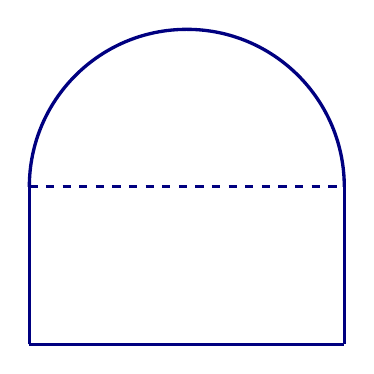
\begin{tikzpicture}
      \draw[very thick,penColor] (2,0) arc (0:180:2 and 2);% top half of ellipse
      \draw[penColor, very thick] (-2,-2) -- (2,-2);
      \draw[penColor, very thick] (2,-2) -- (2,0);
      \draw[penColor,very thick] (-2,-2) -- (-2,0);
      \draw[penColor,very thick,dashed] (-2,0) -- (2,0);
    \end{tikzpicture}
  \end{image}
  If the outer perimeter is $10$ feet, maximize the area. Round your answer to the closest tenth of a square foot.
  \begin{hint}
  Let's label the picture.
   \begin{image}
    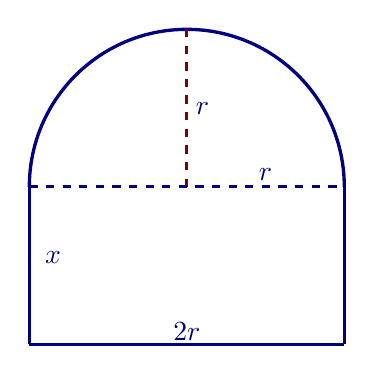
\begin{tikzpicture}
      \draw[very thick,penColor] (2,0) arc (0:180:2 and 2);% top half of ellipse
      \draw[penColor, very thick] (-2,-2) -- (2,-2);
        \draw[penColor2, very thick, dashed] (0,0) -- (0,2);
      \draw[penColor, very thick] (2,-2) -- (2,0);
      \draw[penColor,very thick] (-2,-2) -- (-2,0);
      \draw[penColor,very thick,dashed] (-2,0) -- (2,0);
        \node [below,penColor] at (1,0.35) {$r$};
         \node [below,penColor] at (0.2,1.2) {$r$};
          \node [below,penColor] at (0,-1.6) {$2r$};
           \node [below,penColor] at (-1.7,-0.7) {$x$};
    \end{tikzpicture}
  \end{image}
    \end{hint}
      \begin{hint}
      The outer perimeter, $P$, is given by
      
      $P=2r+2x+r\pi$.
      
      Since we know that $P=10$, we can express $x$ in terms of $r$.
      
      $x=5-r\frac{\pi}{2}-r$.
      
      The area, A , consists of the area of the rectangle + the area of the semicircle:
      
      $A= 2\cdot r\cdot x+\frac{\pi}{2} r^2$
      
        \end{hint}
           \begin{hint}
           We can now express the area  $A$ as a function of $r$:
           
           $A(r)=2\cdot r\cdot (5-r\frac{\pi}{2}-r)+\frac{\pi}{2} r^2=10r-\frac{\pi}{2}r^2-2r^2$.
           
           The domain of A is  the closed interval $\left[0,\frac{10}{2+\pi}\right]$.(Remember: P=10!)
              \end{hint}
                \begin{hint}
                Now we have to find the global maximum of $A$ on its domain.
                First, we have to find the critical points of $A$.
                Since
                
                $A'(r)=10-\pi r-4r$,
                
                it follows that the function $A$ has its only critical point at  $r=\frac{\answer{10}}{4+\pi}$ .
                              \end{hint}
                                \begin{hint}
                                Now, we evaluate $A$ at the end points and at the critical point and then compare the values.
                                
                                $A(0)=0$
                                
                                $A\left(\frac{10}{2+\pi}\right)=\frac{50\pi}{(2+\pi)^2}$
                                
                                $A\left(\frac{\answer{10}}{4+\pi}\right)=\frac{\answer{50}}{4+\pi}\approx 7$
                                
                                This seems complicated. It is better to argue that the derivative 
                                
                                $A'(r)>0$ on $\left(0,\frac{10}{4+\pi}\right)$ and  $A'(r)<0$ on $\left(\frac{10}{4+\pi},\frac{10}{2+\pi}\right)$,
                                
                                 since $A'(r)=10-\pi r-4r=10-r(\pi+4)=-(\pi+4)\left(r-\frac{10}{\pi+4}\right)$.
                                 
                                 
                                 This implies that the global maximum occurs at the critical point.

                                  \end{hint}
  \begin{prompt}
  \[
  A = \answer{7.0} ft^2
  \]
  \end{prompt}
\end{exercise}
\end{document}
